% Runtime results
\section{Performance of EMS-GT with speedup techniques}
Every runtime evaluation using these speedup techniques was run using Intel Xeon, 2.10 Ghz machine. The performance of each algorithm was averaged over 20 synthetic datasets for each $(l, d)$-challenge instance where $l \leq 17$. This section shows the runtime performance of EMS-GT with different combinations of speedup techniques introduced in this study. The version of EMS-GT that yielded the faster runtime performance was used in the proposed EMS-GT2 algorithm. Overall, these speedup techniques improved the runtime performance of EMS-GT algorithm with at least 15\%, 20.37\%, 5.87\%, 6.50\% and 5.17\% for (9, 2), (11, 3), (13, 4), (15, 5) and (17, 6) challenge instances respectively. 


% -------------------------------------------------------------------------------------------------

	\subsection{Evaluation of block boolean flag (BBF) technique}
	% Explanation
	Table \ref{tbl:ems-gt-bf-speedup} shows the runtime performance of block boolean flag technique with its corresponding runtime reductions from the original EMS-GT.

	% Show table
	\begin{table}[h] %speedup_blockmasking
	\renewcommand{\arraystretch}{1.3}
	\centering
	\begin{tabular}{|c|c|c|c|}
	\hline 
	\bfseries\boldmath $(l,d)$ & 
	\bfseries\boldmath EMS-GT & 
	\bfseries\boldmath EMS-GT with BBF & 
	\bfseries \% speedup\\
	\hline
	(9, 2) & 0.0468 s &		0.049 s &	-\\
	(11, 3) & 0.168 s &		0.172 s &	-\\
	(13, 4) & 1.180 s &		1.107 s &	6.21 \%\\
	(15, 5) & 12.767 s &	11.937 s &	6.51 \%\\
	(17, 6) & 143.215 s &	131.776 s &	7.99 \%\\
	\hline\end{tabular}
	
	\caption{EMS-GT with block boolean flags strategy.}
	\label{tbl:ems-gt-bf-speedup}
\end{table}




	% Short analysis
	The block boolean flags technique is efficient when there are significant amount of empty blocks in the candidate motif array. Using this technique, the generation of $d$-neighborhood can focus on those blocks with remaining candidate motifs. 

	Choosing the value for the parameter $n'$ plays a valuable role in this speedup technique. The more sequences processed during the Generation phase the smaller the size of the candidate motifs become and thus the number of empty blocks increases. As we process more sequence in the Generate phase, using the block boolean flags technique, the runtime in generating the $d$-neighborhood of a sequence decreases. Figure \ref{fig:bf-per-sequence-runtime} shows the average runtime in generating the $d$-neighborhood of a sequence per sequence number in (17, 6) problem instance. In evaluating the block boolean flags technique we use $n'=10$, which is the optimum value used also in the previous studies.

	\begin{figure}[h]
	\centering
	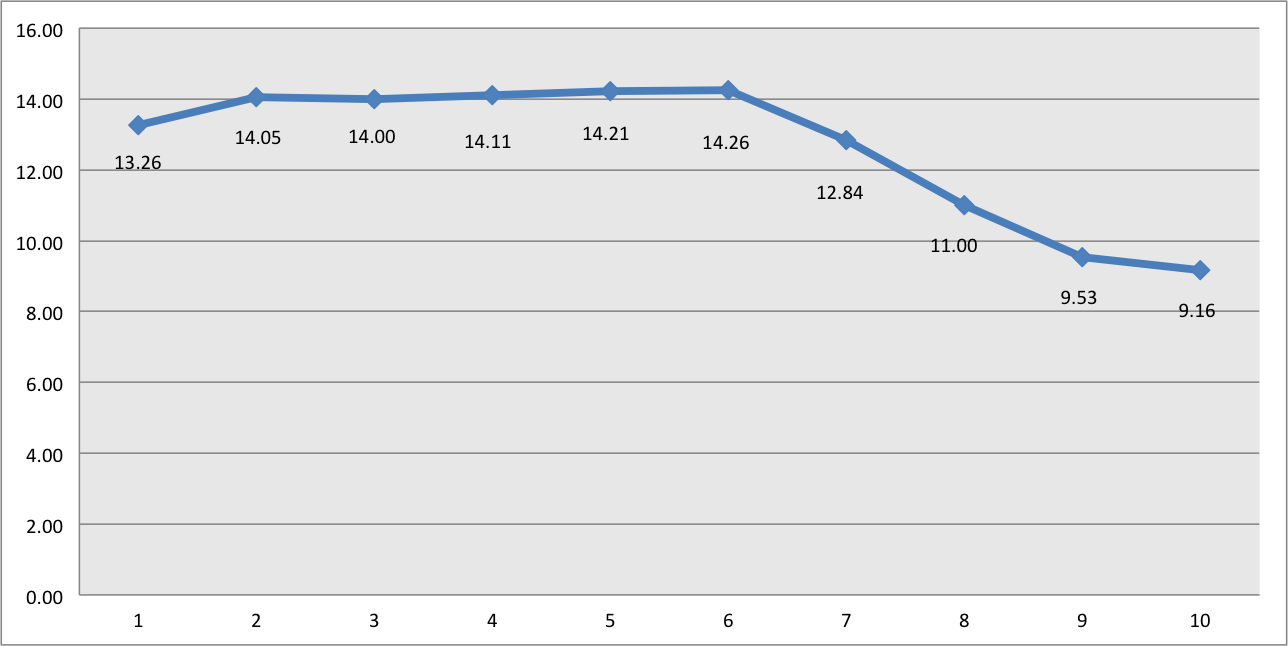
\includegraphics[width=4.5in]{contents/00_images/bf-sequence-runtime}
	\caption{Runtime (s) of $d$-neighborhood generation of sequence for all sequence in Generation Phase using (17, 6) problem instance.}
	\label{fig:bf-per-sequence-runtime}
\end{figure} 

	Additionally, the we incorporated the improved hamming distance computation technique with block boolean flags technique resulting into faster runtime performance, which is shown in Table 4.\ref{tbl:ems-gt-bf-hd-speedup}.

	\begin{table}[h] %speedup_blockmasking
	\renewcommand{\arraystretch}{1.3}
	\centering
	\begin{tabular}{|c|c|c|c|}
	\hline 
	\bfseries\boldmath $(l,d)$ & 
	\bfseries\boldmath EMS-GT & 
	\bfseries\boldmath EMS-GT with BBF and IHD & 
	\bfseries \% speedup\\
	\hline
	(9, 2) & 0.0468 s &		0.035 s 	&	25.00 \%\\
	(11, 3) & 0.168 s &		0.115 s 	&	31.91 \%\\
	(13, 4) & 1.180 s &		0.930 s 	&	21.27 \%\\
	(15, 5) & 12.767 s &	11.532 s  	&	9.68 \%\\
	(17, 6) & 143.215 s &	130.841 s 	&	8.64 \%\\
	\hline\end{tabular}
	
	\caption{EMS-GT with BBF strategy and improved hamming distance computation.}
	\label{tbl:ems-gt-bf-speedup}
\end{table}




% -------------------------------------------------------------------------------------------------

	\subsection{Evaluation of fast candidate motif elimination (FCE) technique}
	Runtime performance of fast candidate motif elimination technique is shown in Table 4.\ref{tbl:ems-gt-fce-speedup}. Fast candidate motif elimination is used the Test phase of the algorithm. This technique is efficient if there are a significant number of candidate motifs left in a block, unlike the block boolean flags technique that is efficient when there are numerous empty blocks in the candidate motifs array. This technique uses different values for $n'$ which are 10, 10, 9, 8 and 7 for the mentioned $(l, d)$ challenge instances respectively. 

	\begin{table}[h] %speedup_blockmasking
	\renewcommand{\arraystretch}{1.3}
	\centering
	\begin{tabular}{|c|c|c|c|}
	\hline 
	\bfseries\boldmath $(l,d)$ & 
	\bfseries\boldmath EMS-GT & 
	\bfseries\boldmath EMS-GT with FCE & 
	\bfseries \% speedup\\
	\hline
	(9, 2) & 0.0468 s &		0.051 s 	&	-\\
	(11, 3) & 0.168 s &		0.172 s 	&	-\\
	(13, 4) & 1.180 s &		1.340 s 	&	-\\
	(15, 5) & 12.767 s &	13.362 s  	&	-\\
	(17, 6) & 143.215 s &	135.799 s 	&	5.17 \%\\
	\hline\end{tabular}
	
	\caption{Runtime comparison of EMS-GT and EMS-GT with fast candidate motif elimination.}
	\label{tbl:ems-gt-fce-speedup}
\end{table}




	EMS-GT with fast candidate motif elimination technique alone only improved the runtime in (17, 6) by 5.17\%, but with the improved hamming distance computation the runtime performance has greatly increased in all of the challenge instances used in the experimentations. The Test phase uses the hamming distance computation heavily and choosing the right sequence to start the Test phase greatly affects the runtime with these speedup techniques. Table 4.\ref{tbl:ems-gt-fce-hd-speedup} shows the runtime performance of EMS-GT with fast candidate motif elimination technique and the improved hamming distance computation.

	\begin{table}[h] %speedup_blockmasking
	\renewcommand{\arraystretch}{1.3}
	\centering
	\begin{tabular}{|c|c|c|c|}
	\hline 
	\bfseries\boldmath $(l,d)$ & 
	\bfseries\boldmath EMS-GT & 
	\bfseries\boldmath EMS-GT with FCE and IHD & 
	\bfseries \% speedup\\
	\hline
	(9, 2) & 0.0468 s &		0.038 s 	&	18.33 \%\\
	(11, 3) & 0.168 s &		0.126 s 	&	25.46 \%\\
	(13, 4) & 1.180 s &		0.946 s 	&	19.88 \%\\
	(15, 5) & 12.767 s &	10.876 s  	&	14.82 \%\\
	(17, 6) & 143.215 s &	111.660 s 	&	22.03 \%\\
	\hline\end{tabular}
	
	\caption{Runtime comparison of EMS-GT and EMS-GT with fast candidate motif elimination and improved hamming distance computation.}
	\label{tbl:ems-gt-fce-hd-speedup}
\end{table}




	Finally, Table 4.\ref{tbl:ems-gt-all-speedup} shows the runtime evaluation of EMS-GT with all of the speedup techniques having $n'$ values used in the fast candidate motif elimination experiments. For all the $(l, d)$ challenge instances used except (17, 6), EMS-GT with fast candidate motif elimination and improved hamming distance computation is still faster than EMS-GT with all speedup techniques. EMS-GT with all speedup techniques failed to compensate for the computational overhead it has introduced in the block boolean flags technique. Given this result, we used the fast candidate motif elimination and improved hamming distance computation only in the proposed EMS-GT2 algorithm.

	\begin{table}[h] %speedup_blockmasking
	\renewcommand{\arraystretch}{1.3}
	\centering
	\begin{tabular}{|c|c|c|c|}
	\hline 
	\bfseries\boldmath $(l,d)$ & 
	\bfseries\boldmath EMS-GT & 
	\bfseries\boldmath EMS-GT with FCE, BFF and IHD & 
	\bfseries \% speedup\\
	\hline
	(9, 2) & 0.0468 s &		0.040 s 	&	15.0 \%\\
	(11, 3) & 0.168 s &		0.134 s 	&	20.37 \%\\
	(13, 4) & 1.180 s &		1.112 s 	&	5.88 \%\\
	(15, 5) & 12.767 s &	11.252 s  	&	11.87 \%\\
	(17, 6) & 143.215 s &	111.634 s 	&	22.05 \%\\
	\hline\end{tabular}
	
	\caption{Runtime comparison of EMS-GT and EMS-GT with all speedup techniques.}
	\label{tbl:ems-gt-all-speedup}
\end{table}




% -------------------------------------------------------------------------------------------------


\section{Runtime performance comparison of EMS-GT2, EMS-GT and qPMS9}
The EMS-GT2, EMS-GT and qPMS9 were evaluated in terms of actual runtime on an Intel Xeon, 2.10 Ghz machine. The performance of each algorithm was averaged over synthetic datasets for each $(l, d)$-challenge isntance where $l \leq 17$. Table 4.\ref{tbl:final-results-ems} shows the runtime results between EMS-GT2 vs EMS-GT while Table 4.\ref{tbl:final-results} shows the runtime results between EMS-GT2 vs the algorithm qPMS9.


\begin{table}[h] %speedup_blockmasking
	\renewcommand{\arraystretch}{1.3}
	\centering
	\begin{tabular}{|c|c|c|c|}
	\hline 
	\bfseries\boldmath $(l,d)$ & 
	\bfseries EMS-GT & 
	\bfseries\boldmath EMS-GT2  & 
	\bfseries \% speedup\\
	\hline
	 (9,2) 	&  0.047 s &    0.038 s &    18.33 \%\\
	(11,3) &   0.168 s &    0.126 s &    25.46 \%\\
	(13,4) &   1.181 s &    0.946 s &   19.88 \%\\
	(15,5) &  12.768 s &   10.876 s &   14.81 \%\\
	(17,6) & 143.215 s &  111.660 s &   22.03 \%\\
	\hline\end{tabular}
	
	\caption{EMS-GT and EMS-GT2 runtime evaluation.}
	\label{tbl:final-results-ems}
\end{table}


% Explanation for Table final-results-ems
The additional speedup techniques become more effective as the $l$ value in the $(l, d)$-instance grows. For every $(l, d)$-challenge instances mentioned, EMS-GT2 has improved the runtime over the EMS-GT for at least 14.8\%. 

\begin{table}[h] %speedup_blockmasking
	\renewcommand{\arraystretch}{1.3}
	\centering
	\begin{tabular}{|c|c|c|c|}
	\hline 
	\bfseries\boldmath $(l,d)$ & 
	\bfseries qPMS9 & 
	\bfseries\boldmath EMS-GT2 & 
	\bfseries \% speedup\\
	\hline
	 (9,2) &   0.647 s &    0.039 s &   93.97 \%\\
	(11,3) &   1.276 s &    0.140 s &   89.02 \%\\
	(13,4) &   4.269 s &    0.758 s &   82.24 \%\\
	(15,5) &  24.737 s &   10.565 s &   57.29 \%\\
	(17,6) & 118.226 s &  112.311 s &   5.00 \%\\
	\hline\end{tabular}
	
	\caption{EMS-GT2 and qPMS9 runtime evaluation.}
	\label{tbl:final-results}
\end{table}




% Explanation for Table final-results
Previous implementations of EMS-GT failed to beat qPMS9 in $(17, 6)$-challenge instance. The proposed EMS-GT2 not only produces improved runtimes but also succeed in beating the qPMS9 in all of the $(l, d)$-challenge instances where $l \leq 17$. Even though the implementation of EMS-GT can only run in $(l, d)$-challenge instances where $l \leq 17$ because of computer memory constraint, studies have shown that typical length of motifs is around 10 base pairs (bp) \cite{stewart2012transcription}.





